\documentclass[12pt,letterpaper]{article}
\usepackage{pdfpages}
\usepackage{fancyhdr}
\usepackage[colorlinks=true, urlcolor=blue, linkcolor=blue]{hyperref}
\usepackage{graphicx}
\usepackage[top=1.4in, left=0.5in, right=0.5in, bottom=0.8in]{geometry}
\usepackage[T1]{fontenc}
\usepackage{helvet}
\pagestyle{fancy}
\renewcommand{\headrulewidth}{0pt}
\renewcommand{\footrulewidth}{0pt}
\setlength{\parindent}{0em}
\setlength{\parskip}{1em}


\fancyfoot[C]{\setlength{\unitlength}{1in}\begin{picture}(5,0)\put(-1.8,-1){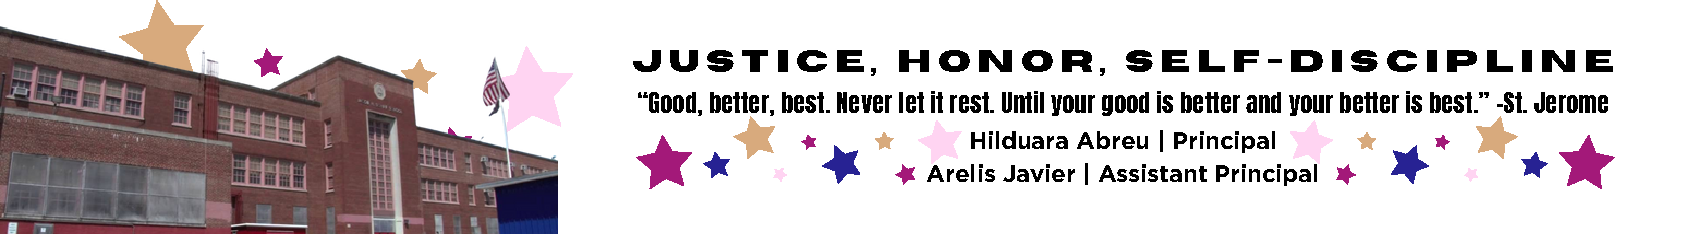
\includegraphics[width=8.8in,height=1.3in]{logo-1}}\end{picture}}
\fancyhead[C]{\setlength{\unitlength}{1in}\begin{picture}(5,0)\put(-1.9,-1){
\includegraphics[width=8.9in,height=1.3in]{logo-2}}\end{picture}}

\pagenumbering{gobble}
\addtolength{\evensidemargin}{-2in}
\addtolength{\topmargin}{-0.5in}
\addtolength{\textwidth}{0in}
%%%%%%%%%%%%%%%%%%%%%%%%%%%%%%%%%%%%%%%%%%%%%%%%%%%%%%%%%%%%%%%%%%

\begin{document}
\vspace*{0.5in}
School Website: \href{https://www.ps192.org}{www.ps192.org}

\textbf{Principal's Message March 2024}

Dear Parents or Guardians,

As we welcome the arrival of March, I am pleased to share with you the schedule of upcoming events and activities for the month.

Please mark your calendars for the following:
\begin{itemize}
\item Graduation Pictures: March 5th
\item Parent-Teacher Conferences: Thursday, March 7th (By appointment only)
\item Parent Association Meeting: Tuesday, March 12th, at 8:30 a.m. in the Library
\item SLT: Friday, March 15th, at 2:30 p.m. in the Library
\item Camps Meeting: Thursday, March 21st, at 8:00 a.m. in the Library
\item Coffee with the Principal: Thursday, March 28th, at 8:00 a.m. in the Library 
\end{itemize}
Tips for Attending the PS 192 Virtual Parent-Teacher Conference
\begin{itemize}
\item Test Your Technology: Before the conference, ensure your device, microphone, and camera are working properly. Check your internet connection to avoid any disruptions during the meeting.
\item Create a Quiet Space: Find a quiet, private area in your home where you can speak freely and listen without distractions.
\item Be Punctual: Log in to the virtual meeting a few minutes early to resolve any last-minute technical issues and be ready when the conference starts.
\item Review Your Child’s Progress: Look over your child’s assignments, report cards, and any teacher feedback. Note any areas you’d like to discuss or need clarification on.
\item Prepare Questions: Write down questions or topics you want to cover. Prioritize them in case time runs short.
\item Stay Focused: Keep the conversation on your child’s academic and social development. Virtual meetings can feel less personal, so staying on topic is key.
\pagebreak
\vspace*{.5in}
\item Take Notes: Have a pen and paper ready, or use a digital note-taking app to record important points and suggestions from the teacher.
\item Use a Headset: If possible, use a headset with a microphone for better sound quality and to minimize background noise.
\item Follow Virtual Meeting Etiquette: Mute your microphone when not speaking, use the “raise hand” feature if available, and be mindful of the time allotted for your conference.
\item Discuss Next Steps: Ask about ways to support your child’s learning at home and set up a plan for follow-up communication with the teacher.
\item Express Appreciation: Thank the teacher for their time and effort, and acknowledge the unique challenges of teaching in a virtual environment.
\item Review the Meeting: After the conference, go over your notes and discuss the meeting with your child, focusing on positive points and areas for growth.
\end{itemize}

I would like to emphasize the significance of the Parent-Teacher Conferences. This is an invaluable occasion to gain insights into your child’s progress and to engage in meaningful dialogue about their educational journey. Education is a dynamic and sometimes challenging adventure, and maintaining open communication with your child’s teachers is key to navigating it successfully.

Our dedicated teachers are always ready to listen and collaborate on strategies to support your child’s academic achievements. I eagerly anticipate meeting with you during the conferences.
Please also remember that teachers are available for consultation every Tuesday from 2:20 p.m. to 3:00 p.m. following dismissal. This is an excellent time to discuss your child’s performance and any other pertinent matters.

Your involvement and support are crucial to the success of our school’s events and activities. 

Thank you for your continued partnership.

Warm regards, 


\includegraphics[width=0.12\textwidth]{hil_signature}

\textbf{Hilduara Abreu}

\textbf{Principal P.S. 192}

\textit{The School of Joyful Learning!}

\newpage
\vspace*{.5in}
Nuestro Sitio Web: \href{https://www.ps192.org}{www.ps192.org}

\textbf{Mensaje de La Directora Para Marzo 2024}

Estimados padres o tutores,

Mientras damos la bienvenida a la llegada de marzo, me complace compartir con ustedes el calendario de próximos eventos y actividades para el mes.

Por favor marque sus calendarios para lo siguiente:
\begin{itemize}
\item Fotos de graduación: 5 de marzo
\item Conferencias de padres y maestros: jueves 7 de marzo (solo con cita previa)
\item Reunión de la Asociación de Padres: martes 12 de marzo a las 8:30 a.m. en la Biblioteca
\item SLT: viernes 15 de marzo, a las 14:30 horas. en la biblioteca
\item Reunión de Campamentos: jueves 21 de marzo a las 8:00 a.m. en la Biblioteca
\item Café con el Director: jueves 28 de marzo a las 8:00 a.m. en la Biblioteca
\end{itemize}
Consejos para asistir a la conferencia virtual de padres y maestros de PS 192
\begin{itemize}
\item Pruebe su tecnología: antes de la conferencia, asegúrese de que su dispositivo, micrófono y cámara funcionen correctamente. Verifique su conexión a Internet para evitar interrupciones durante la reunión.
\item Cree un espacio tranquilo: encuentre un área tranquila y privada en su hogar donde pueda hablar libremente y escuchar sin distracciones.
\item Sea puntual: inicie sesión en la reunión virtual unos minutos antes para resolver cualquier problema técnico de último momento y esté listo cuando comience la conferencia.
\item Revise el progreso de su hijo: revise las tareas, las boletas de calificaciones y los comentarios de los maestros de su hijo. Anota cualquier área que quieras discutir o sobre la que necesites una aclaración.
\item Prepare preguntas: escriba las preguntas o temas que desee cubrir. Priorízalos en caso de que el tiempo se acabe.
\item Manténgase enfocado: mantenga la conversación sobre el desarrollo académico y social de su hijo. Las reuniones virtuales pueden parecer menos personales, por lo que mantenerse en el tema es clave.
\pagebreak
\vspace*{.5in}
\item Tomar notas: tenga a mano papel y lápiz, o utilice una aplicación de toma de notas digital para registrar puntos importantes y sugerencias del profesor.
\item Utilice unos auriculares: si es posible, utilice unos auriculares con micrófono para obtener una mejor calidad de sonido y minimizar el ruido de fondo.
\item Siga la etiqueta de la reunión virtual: silencie su micrófono cuando no esté hablando, use la función "levantar la mano" si está disponible y tenga en cuenta el tiempo asignado para su conferencia.
\item Discuta los próximos pasos: pregunte sobre formas de apoyar el aprendizaje de su hijo en casa y establezca un plan para la comunicación de seguimiento con el maestro.
\item Agradecimiento Expreso: Agradezca al maestro por su tiempo y esfuerzo, y reconozca los desafíos únicos de la enseñanza en un entorno virtual.
\item Revise la reunión: Después de la conferencia, revise sus notas y analice la reunión con su hijo, centrándose en los puntos positivos y las áreas de crecimiento.
\end{itemize}

Me gustaría enfatizar la importancia de las conferencias de padres y maestros. Esta es una ocasión invaluable para obtener información sobre el progreso de su hijo y entablar un diálogo significativo sobre su trayectoria educativa. La educación es una aventura dinámica y, a veces, desafiante, y mantener una comunicación abierta con los maestros de su hijo es clave para afrontarla con éxito.

Nuestros dedicados maestros siempre están listos para escuchar y colaborar en estrategias para apoyar los logros académicos de su hijo. Anticipo ansiosamente reunirme con usted durante las conferencias.
Recuerde también que los profesores están disponibles para consulta todos los martes de 2:20 PM  a 3:00 PM siguiente a la hora de salida. Este es un momento excelente para hablar sobre el desempeño de su hijo y cualquier otro asunto pertinente.

Su participación y apoyo son cruciales para el éxito de los eventos y actividades de nuestra escuela.

Gracias por su continua colaboración.

Un cordial saludo,


\includegraphics[width=0.12\textwidth]{hil_signature}

\textbf{Hilduara Abreu}

\textbf{Principal P.S. 192}

\textit{The School of Joyful Learning!}
\end{document}
